\section{Additional Results}\label{app:allresults}

This section contains additional results that were not displayed in the main paper.

Tables~\ref{tab:pretxpredfull} and ~\ref{tab:pretxpredfullcc} presents the full model validation results that also include estimators using the Oaxaca-Blinder OLS and GLS weights (see, e.g, \cite{kline2011oaxaca}). The first table only presents the RMSE, with rows ordered by RMSE for each dataset, while the second table contains the numbers for each individual year and the RMSE. The rows are ordered by RMSE on the primary dataset. We find that these estimators perform quite poorly, again showing that the cost of extrapolation is quite high in our application. 

Table~\ref{tab:confintmain} displays the point estimates and confidence intervals from all estimators we considered, including those using the ``heterogeneous adjustment.''

Figure~\ref{fig:loostateplot} displays the change in our estimator when removing each state for all four of our estimators on the adjusted dataset (``homogeneous'') and the unadjusted dataset (``unadjusted'') for the primary dataset. Figure~\ref{fig:loostateplotc2} displays the same information when excluding the early expansion states. 

Our final two tables (Tables~\ref{tab:loojackknifec1} and \ref{tab:loojackknifec2}) display each point estimate associated with each estimator in the leave-one-state-out jackknife.

\begin{table}
\centering
\begin{threeparttable}\caption{Estimator pre-treatment outcome RMSE (in \% points)}\label{tab:pretxpredfullcc}
\begin{tabular}{llrllr}
\hline
\multicolumn{3}{c}{Primary data} & \multicolumn{3}{c}{Early expansion 
 excluded} \\ 
 \hline
% \cmidrule(lr){1-3} \cmidrule(lr){4-6}
Sigma estimate & Estimator & RMSE & Sigma estimate & Estimator & RMSE \\ 
\hline
Homogeneous & SBW & 0.20 & Homogeneous & BC-HSBW & 0.07 \\ 
Homogeneous & H-SBW & 0.23 & Homogeneous & BC-SBW & 0.12 \\ 
Heterogeneous & SBW & 0.27 & Heterogeneous & BC-HSBW & 0.14 \\ 
Heterogeneous & H-SBW & 0.36 & Heterogeneous & BC-SBW & 0.15 \\ 
Homogeneous & BC-SBW & 0.39 & Homogeneous & H-SBW & 0.25 \\ 
Heterogeneous & BC-SBW & 0.42 & Homogeneous & SBW & 0.26 \\ 
Unadjusted & SBW & 0.56 & Heterogeneous & SBW & 0.28 \\ 
Unadjusted & H-SBW & 0.57 & Heterogeneous & H-SBW & 0.29 \\ 
Homogeneous & BC-HSBW & 0.58 & Heterogeneous & GLS & 0.29 \\ 
Heterogeneous & BC-HSBW & 0.63 & Heterogeneous & OLS & 0.39 \\ 
Unadjusted & BC-SBW & 0.88 & Unadjusted & SBW & 0.42 \\ 
Unadjusted & OLS & 0.88 & Unadjusted & H-SBW & 0.46 \\ 
Unadjusted & GLS & 0.89 & Unadjusted & BC-HSBW & 0.60 \\ 
Unadjusted & BC-HSBW & 0.96 & Unadjusted & GLS & 0.63 \\ 
Homogeneous & OLS & 1.50 & Unadjusted & OLS & 0.71 \\ 
Homogeneous & GLS & 1.61 & Unadjusted & BC-SBW & 0.71 \\ 
Heterogeneous & GLS & 12.47 & Homogeneous & GLS & 0.98 \\ 
Heterogeneous & OLS & 16.21 & Homogeneous & OLS & 1.10 \\ 
 \hline
\end{tabular}
\end{threeparttable}
\end{table}

\begin{table}
    \centering
\begin{threeparttable}\caption{Estimator pre-treatment outcome prediction error (in \% points)}\label{tab:pretxpredfull}
\begin{tabular}{llrrr|rrr}\\ \hline
 &  & \multicolumn{3}{c}{Primary data} & \multicolumn{3}{c}{Early expansion 
 excluded} \\
 \hline
 %\cmidrule(lr){3-5} \cmidrule(lr){6-8}
Sigma estimate & Estimator & 2012 error & 2013 error & RMSE & 2012 error & 2013 error & RMSE \\ 
\hline
Homogeneous & SBW & -0.18 & -0.22 & 0.20 & 0.32 & -0.18 & 0.26 \\ 
Homogeneous & H-SBW & -0.24 & -0.21 & 0.23 & 0.26 & -0.24 & 0.25 \\ 
Heterogeneous & SBW & -0.25 & -0.30 & 0.27 & 0.31 & -0.24 & 0.28 \\ 
Heterogeneous & H-SBW & -0.32 & -0.39 & 0.36 & 0.25 & -0.32 & 0.29 \\ 
Homogeneous & BC-SBW & -0.42 & -0.35 & 0.39 & 0.09 & -0.15 & 0.12 \\ 
Heterogeneous & BC-SBW & -0.45 & -0.39 & 0.42 & 0.07 & -0.21 & 0.15 \\ 
Unadjusted & SBW & -0.50 & -0.61 & 0.56 & -0.18 & -0.56 & 0.42 \\ 
Unadjusted & H-SBW & -0.52 & -0.61 & 0.57 & -0.26 & -0.60 & 0.46 \\ 
Homogeneous & BC-HSBW & -0.53 & -0.62 & 0.58 & 0.05 & -0.09 & 0.07 \\ 
Heterogeneous & BC-HSBW & -0.53 & -0.72 & 0.63 & 0.03 & -0.19 & 0.14 \\ 
Unadjusted & BC-SBW & -0.82 & -0.93 & 0.88 & -0.55 & -0.84 & 0.71 \\ 
Unadjusted & OLS & -0.91 & -0.84 & 0.88 & -0.81 & -0.59 & 0.71 \\ 
Unadjusted & GLS & -0.87 & -0.91 & 0.89 & -0.78 & -0.44 & 0.63 \\ 
Unadjusted & BC-HSBW & -0.93 & -0.99 & 0.96 & -0.61 & -0.58 & 0.60 \\ 
Homogeneous & OLS & -1.75 & -1.21 & 1.50 & 1.12 & -1.08 & 1.10 \\ 
Homogeneous & GLS & -1.76 & -1.45 & 1.61 & 1.22 & -0.66 & 0.98 \\ 
Heterogeneous & GLS & -1.18 & -17.60 & 12.47 & 0.27 & -0.32 & 0.29 \\ 
Heterogeneous & OLS & -0.85 & -22.90 & 16.21 & 0.22 & -0.50 & 0.39 \\ 
 \hline
 \end{tabular}
\end{threeparttable}
\end{table}

\begin{table}[h!]
\centering
\begin{threeparttable}
\caption{Point estimates and confidence intervals: all estimators}
%\begin{longtable}{llrrrrrr}
\label{tab:confintmain}
\begin{tabular}{lllrlr}
\hline
 &  & \multicolumn{2}{c}{Primary data} & \multicolumn{2}{c}{Early expansion 
 excluded} \\
  \hline
Weight type & Adjustment & Estimate (95\% CI) & Difference & Estimate (95\% CI) & Difference \\ 
  \hline
H-SBW & Homogeneous & -2.33 (-3.54, -1.11) & 0.01 & -2.09 (-3.24, -0.94) & 0.19 \\ 
  H-SBW & Heterogeneous & -2.24 (-3.47, -1.00) & 0.10 & -2.06 (-3.36, -0.77) & 0.22 \\ 
  H-SBW & Unadjusted & -2.34 (-2.88, -1.79) & - & -2.28 (-2.87, -1.70) & - \\ 
  BC-HSBW & Homogeneous & -2.05 (-3.30, -0.80) & 0.17 & -1.94 (-3.27, -0.61) & 0.28 \\ 
  BC-HSBW & Heterogeneous & -1.98 (-3.21, -0.75) & 0.24 & -1.93 (-3.55, -0.32) & 0.29 \\ 
  BC-HSBW & Unadjusted & -2.22 (-2.91, -1.52) & - & -2.22 (-3.14, -1.31) & - \\ 
  SBW & Homogeneous & -2.35 (-3.76, -0.95) & 0.04 & -2.05 (-3.19, -0.91) & 0.16 \\ 
  SBW & Heterogeneous & -2.28 (-3.58, -0.98) & 0.11 & -2.03 (-3.35, -0.72) & 0.18 \\ 
  SBW & Unadjusted & -2.39 (-2.99, -1.79) & - & -2.21 (-2.75, -1.68) & - \\ 
  BC-SBW & Homogeneous & -2.07 (-3.14, -1.00) & 0.13 & -1.99 (-3.33, -0.66) & 0.23 \\ 
  BC-SBW & Heterogeneous & -2.00 (-3.07, -0.92) & 0.20 & -2.00 (-3.65, -0.34) & 0.23 \\ 
  BC-SBW & Unadjusted & -2.19 (-2.94, -1.45) & - & -2.23 (-3.12, -1.33) & - \\ 
   \hline
\end{tabular}
    \begin{tablenotes}
      \item[] Note: ``Difference'' column reflects difference between adjusted and unadjusted estimators
        \item[] Note: Confidence intervals are estimated using the leave-one-state-out jackknife and quantiles from t-distribution with $m_1 - 1$ degrees of freedom.
    \end{tablenotes}
\end{threeparttable}
\end{table}

\begin{figure}[H]
\begin{center}
    \caption{Leave-one-state-out point estimates minus primary estimate, primary dataset}
    \label{fig:loostateplot}
    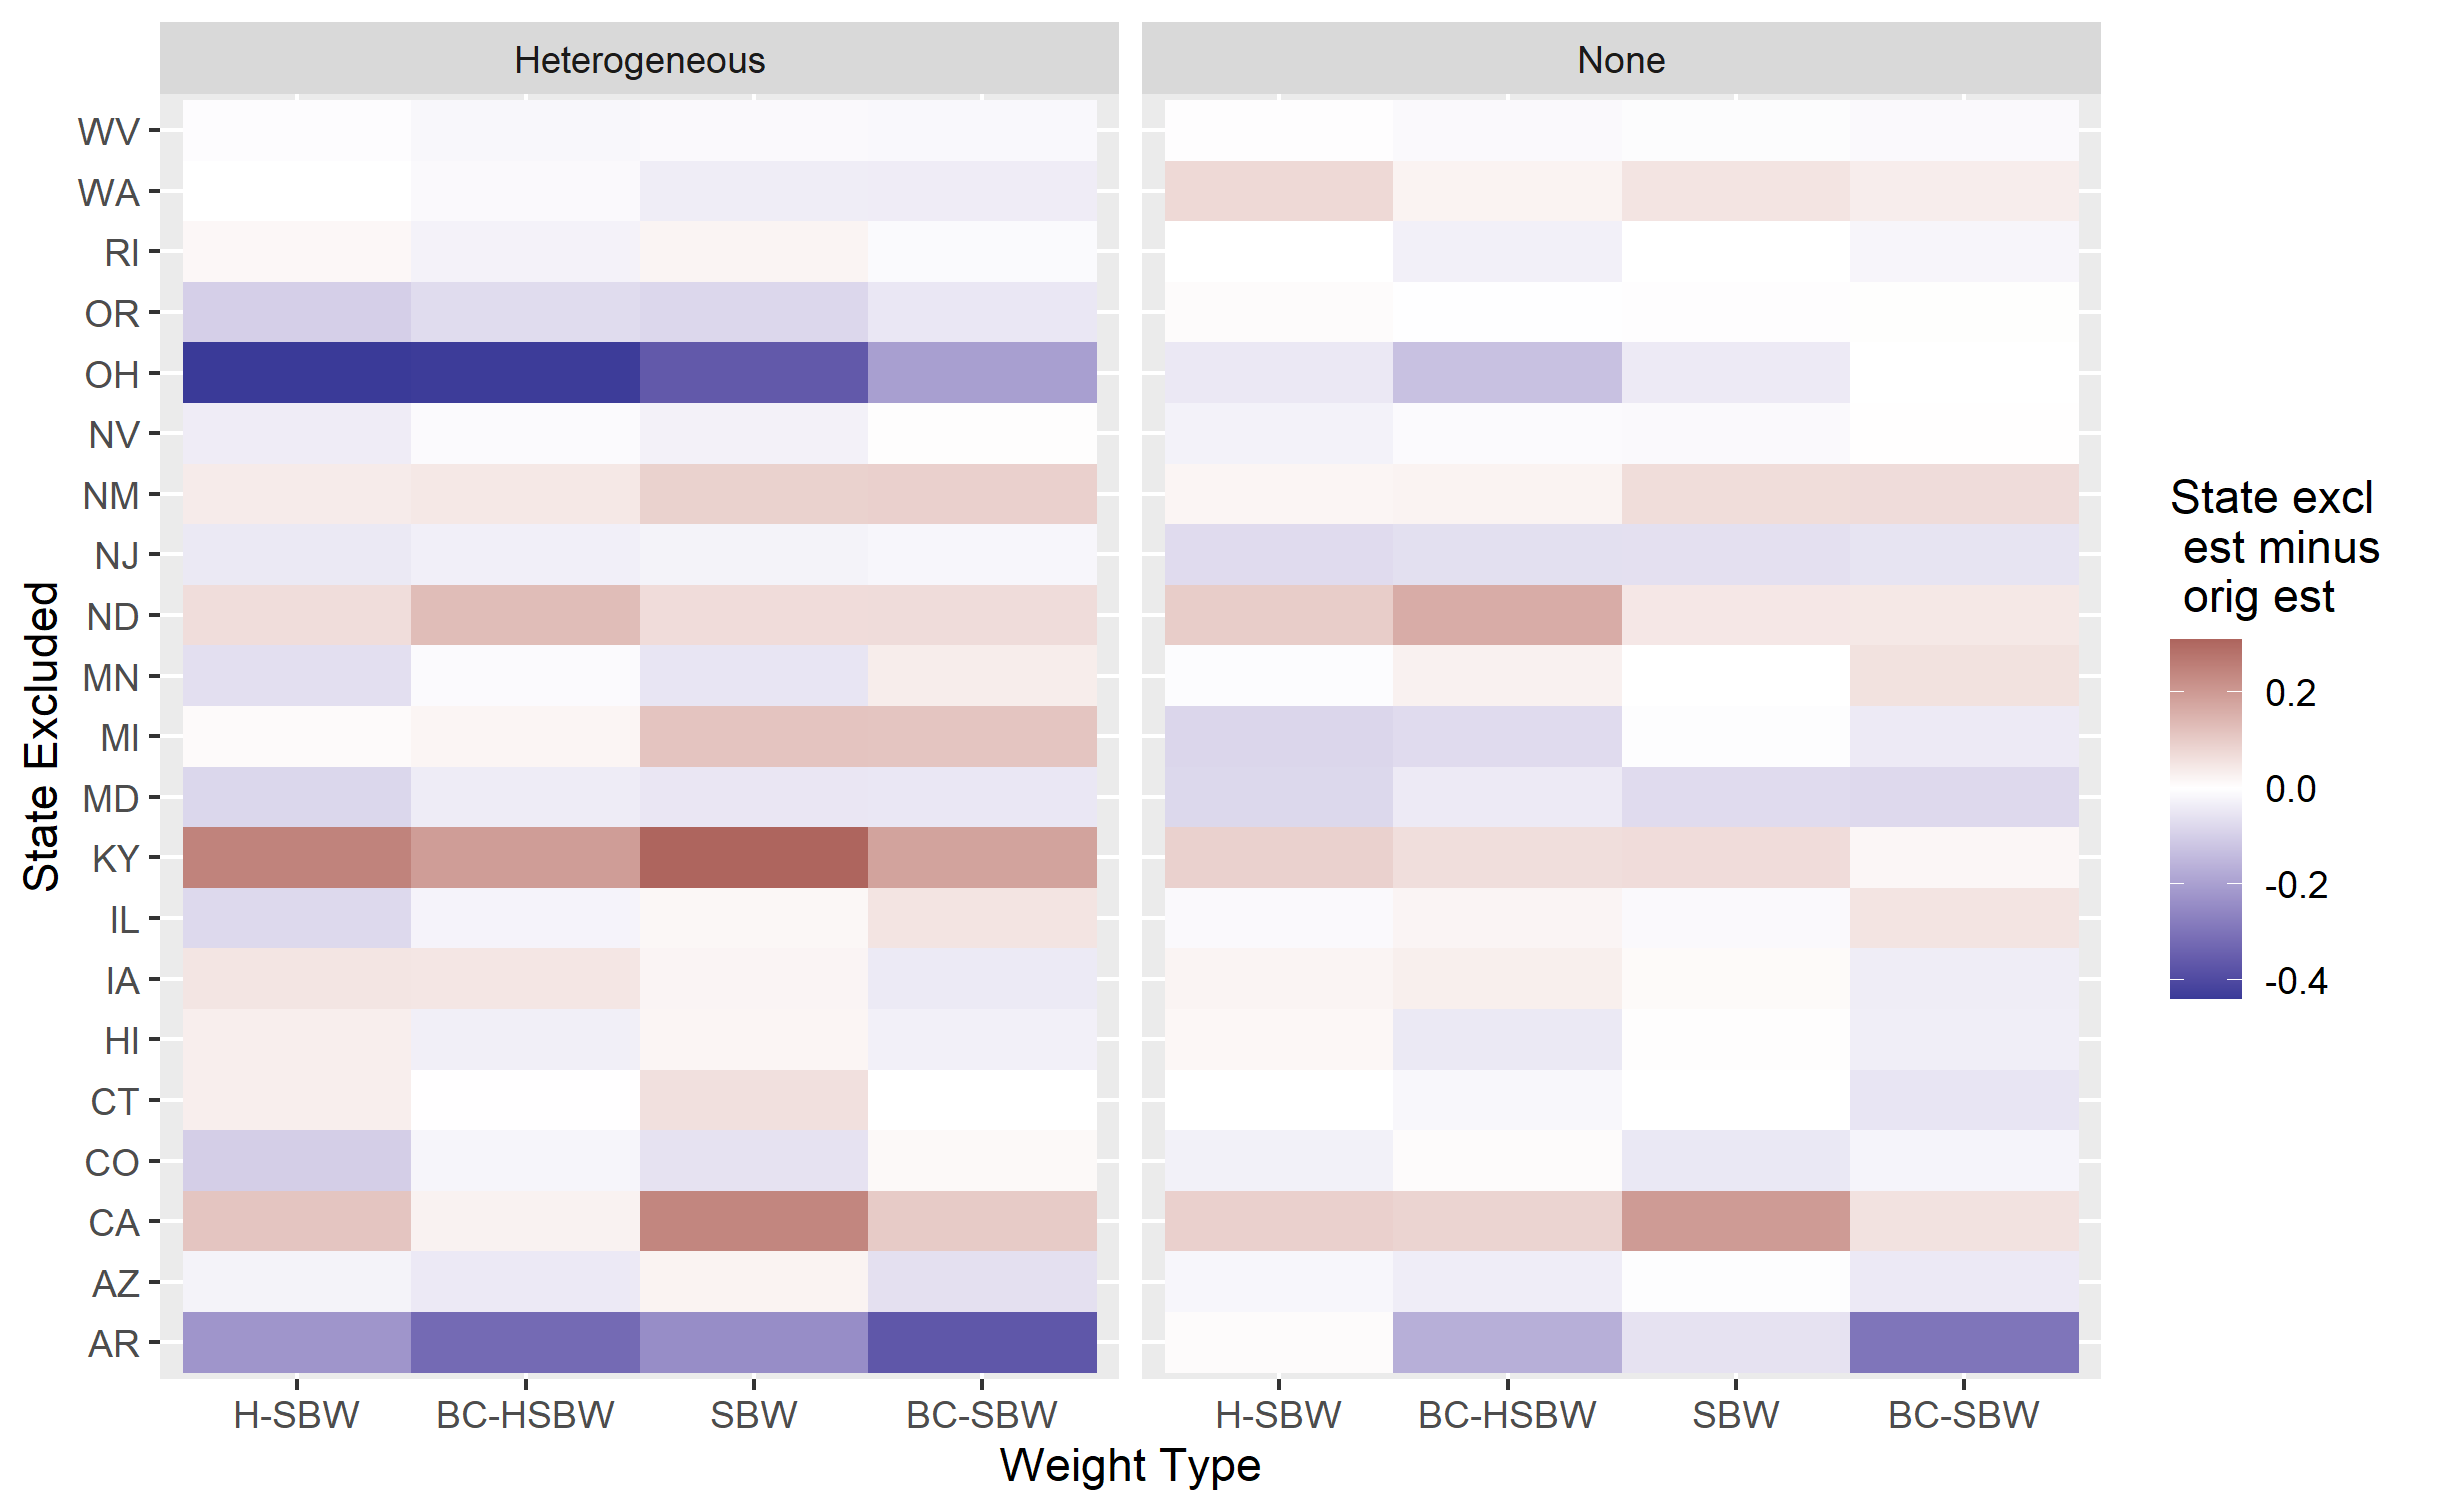
\includegraphics[scale=0.6]{01_Plots/loostate-sensitivityc1-proc-uu-avg.png}
\end{center}
\subcaption{Colors reflect the magnitude of the difference in the estimates when subtracting the original estimate from the estimate that excludes the specified state. The values in the right panel are on the unadjusted data.}
\end{figure}

\begin{figure}[H]
\begin{center}
    \caption{Leave-one-state-out point estimates minus primary estimate, early expansion excluded}
    \label{fig:loostateplotc2}
    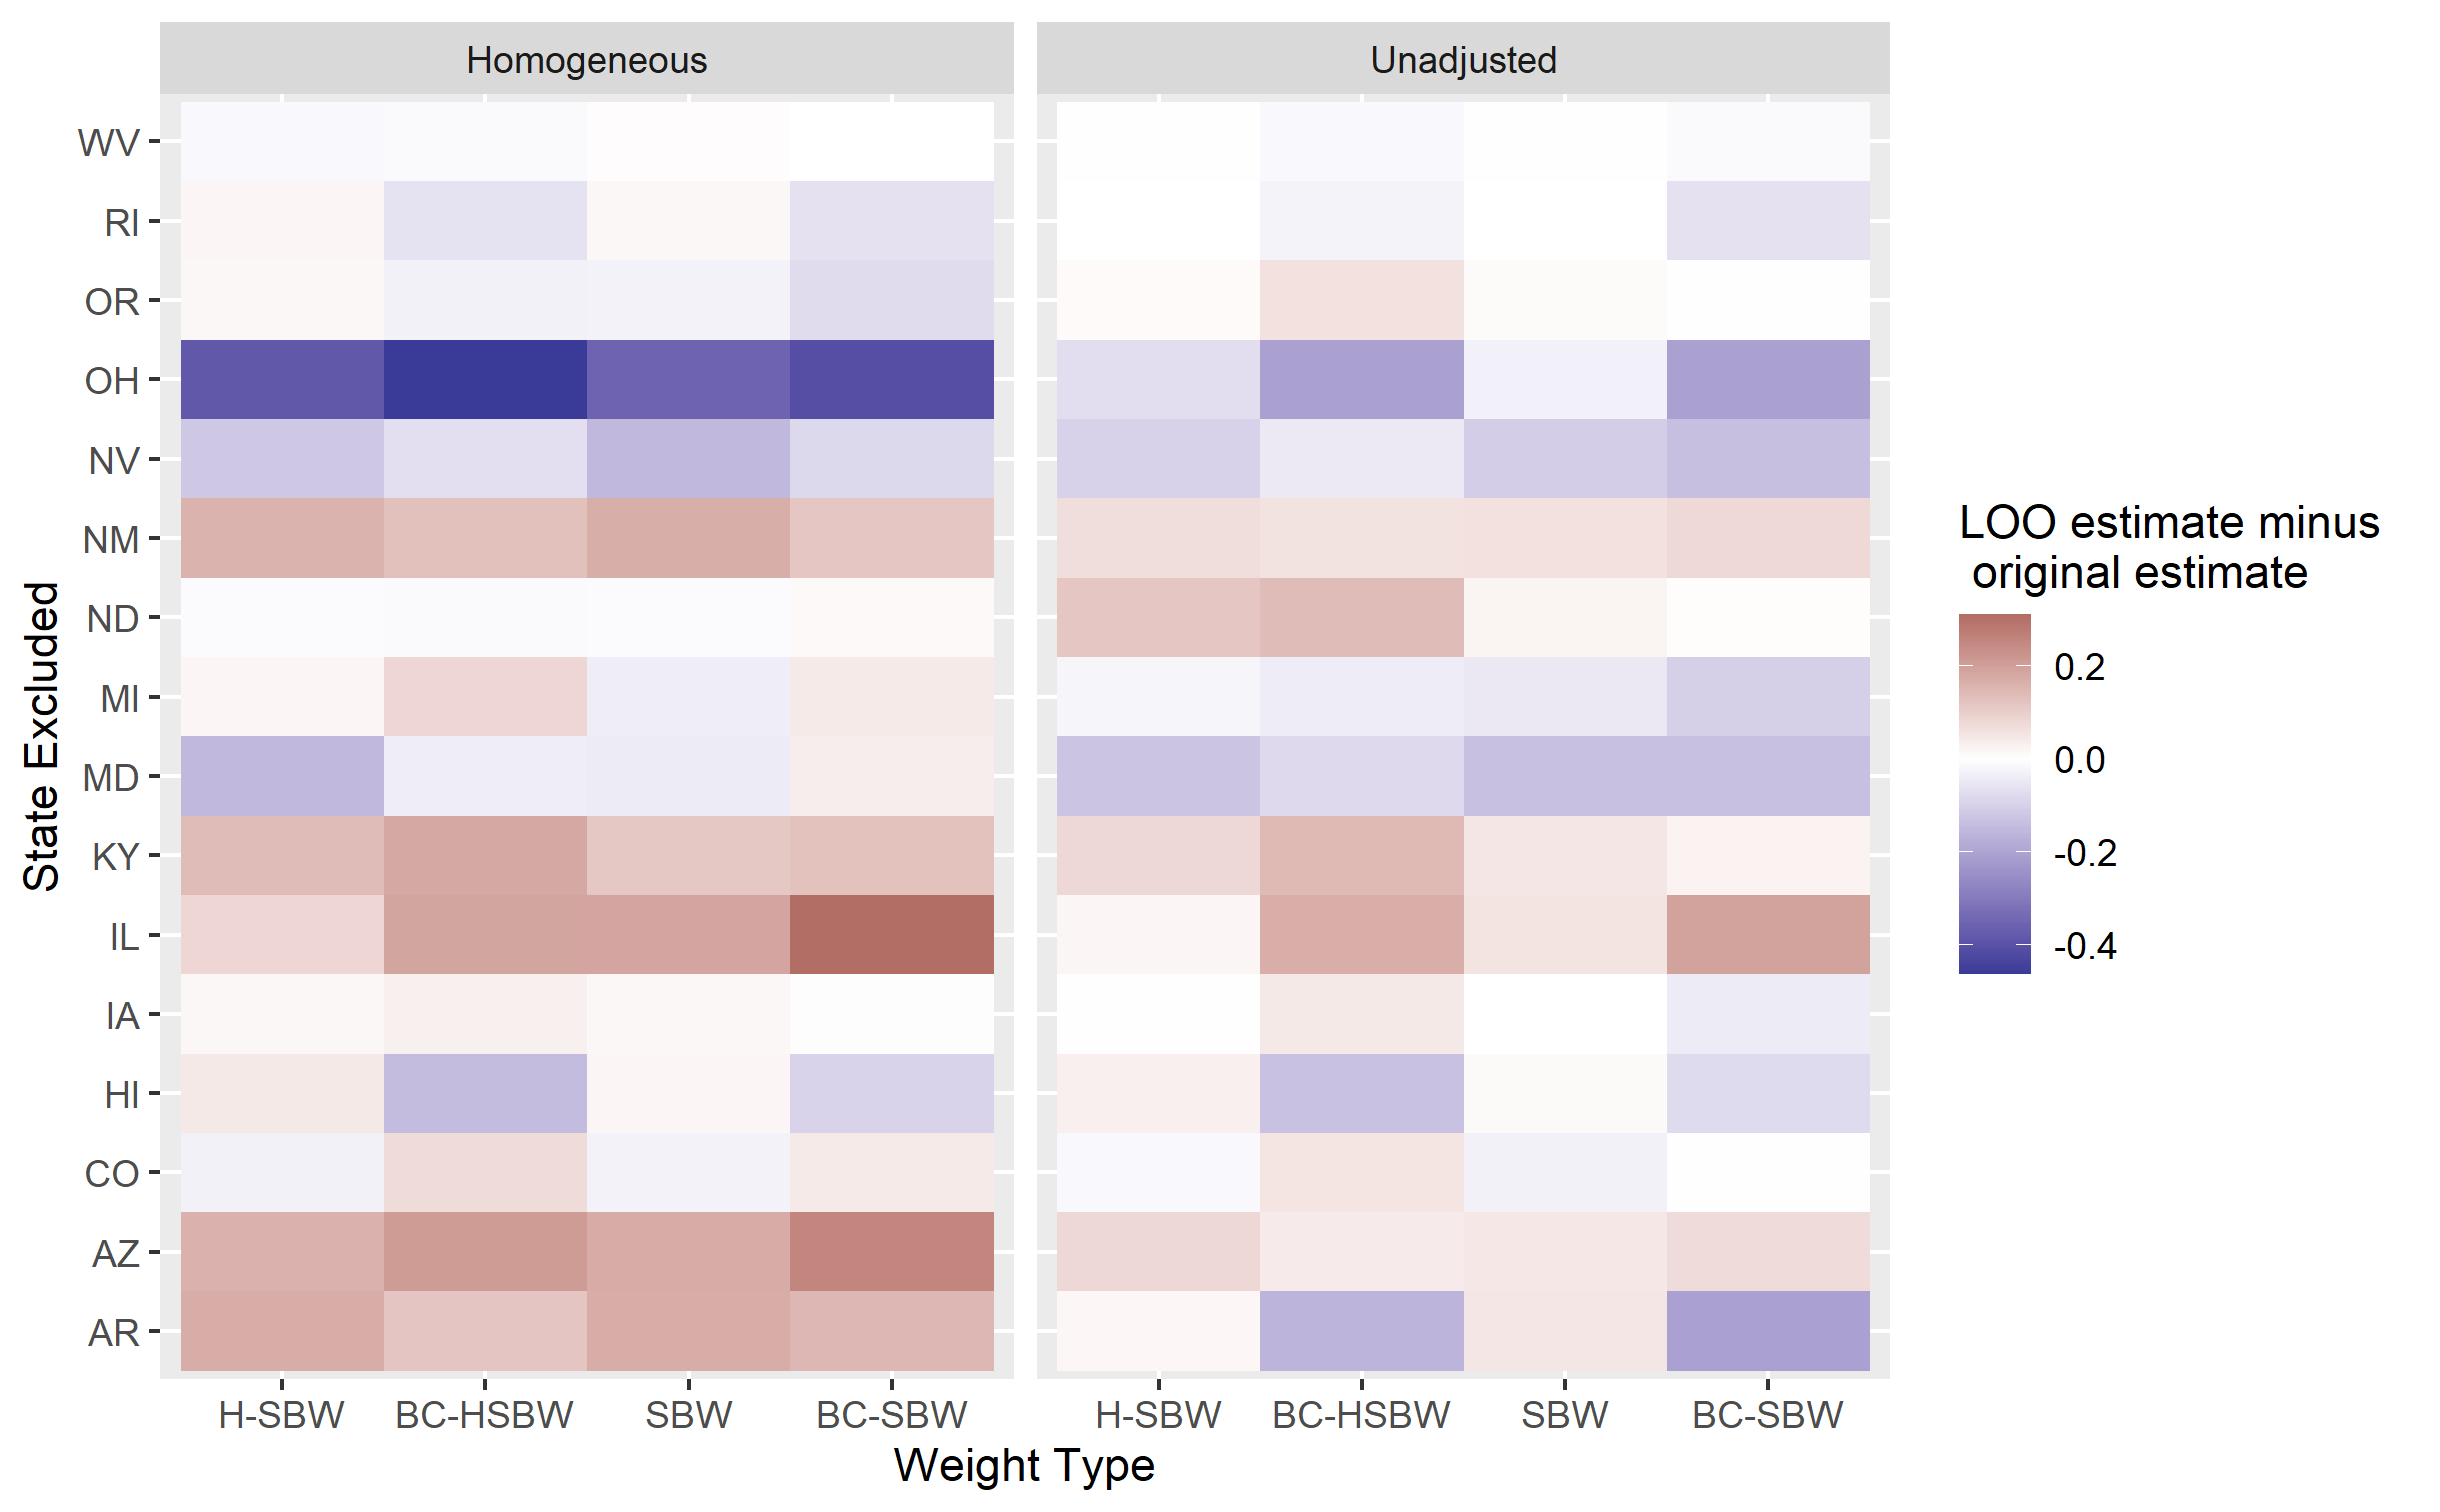
\includegraphics[scale=0.6]{01_Plots/loostate-sensitivityc2-proc-uu-avg.png}
\end{center}
\subcaption{Colors reflect the magnitude of the difference in the estimates when subtracting the original estimate from the estimate that excludes the specified state. The values in the right panel are on the unadjusted data.}
\end{figure}

\begin{landscape}

\begin{table}[H]\caption{Leave one state out jackknife point estimates: all estimators, primary dataset}\label{tab:loojackknifec1}
\centering
%\begin{tabular}
\begin{longtable}{lrrrr|rrrr|rrrr}
\hline
 & \multicolumn{4}{c}{Homogeneous} & \multicolumn{4}{c}{Heterogeneous} & \multicolumn{4}{c}{Unadjusted} \\ 
 \hline
 %\cmidrule(lr){2-5} \cmidrule(lr){6-9} \cmidrule(lr){10-13}
Left out state & BC-HSBW & BC-SBW & H-SBW & SBW & BC-HSBW & BC-SBW & H-SBW & SBW & BC-HSBW & BC-SBW & H-SBW & SBW \\ 
\hline
All & -2.05 & -2.07 & -2.33 & -2.35 & -1.98 & -2.00 & -2.24 & -2.28 & -2.22 & -2.19 & -2.34 & -2.39 \\ 
AR & -2.40 & -2.45 & -2.59 & -2.61 & -2.30 & -2.36 & -2.46 & -2.52 & -2.38 & -2.49 & -2.33 & -2.45 \\ 
AZ & -2.06 & -2.14 & -2.28 & -2.31 & -2.02 & -2.06 & -2.26 & -2.25 & -2.25 & -2.24 & -2.35 & -2.39 \\ 
CA & -1.94 & -1.93 & -2.17 & -2.08 & -1.96 & -1.90 & -2.12 & -2.04 & -2.13 & -2.14 & -2.24 & -2.19 \\ 
CO & -2.02 & -2.03 & -2.34 & -2.34 & -2.00 & -1.98 & -2.34 & -2.34 & -2.21 & -2.22 & -2.36 & -2.44 \\ 
CT & -2.04 & -2.07 & -2.27 & -2.28 & -1.98 & -2.00 & -2.20 & -2.22 & -2.23 & -2.25 & -2.34 & -2.39 \\ 
HI & -2.08 & -2.09 & -2.30 & -2.33 & -2.01 & -2.03 & -2.20 & -2.26 & -2.26 & -2.23 & -2.32 & -2.39 \\ 
IA & -2.01 & -2.10 & -2.29 & -2.34 & -1.93 & -2.04 & -2.18 & -2.26 & -2.19 & -2.23 & -2.31 & -2.38 \\ 
IL & -2.04 & -1.98 & -2.36 & -2.29 & -2.00 & -1.94 & -2.31 & -2.26 & -2.20 & -2.14 & -2.35 & -2.40 \\ 
KY & -1.83 & -1.85 & -2.03 & -1.99 & -1.79 & -1.82 & -1.99 & -1.97 & -2.15 & -2.18 & -2.25 & -2.32 \\ 
MD & -2.06 & -2.11 & -2.40 & -2.40 & -2.02 & -2.04 & -2.32 & -2.33 & -2.26 & -2.27 & -2.42 & -2.46 \\ 
MI & -2.03 & -2.02 & -2.31 & -2.29 & -1.96 & -1.88 & -2.23 & -2.16 & -2.29 & -2.24 & -2.42 & -2.39 \\ 
MN & -2.02 & -2.03 & -2.34 & -2.38 & -1.99 & -1.96 & -2.30 & -2.33 & -2.19 & -2.14 & -2.34 & -2.39 \\ 
ND & -1.93 & -2.01 & -2.26 & -2.29 & -1.85 & -1.93 & -2.17 & -2.21 & -2.05 & -2.15 & -2.24 & -2.34 \\ 
NJ & -2.04 & -2.04 & -2.32 & -2.33 & -2.01 & -2.01 & -2.28 & -2.30 & -2.28 & -2.25 & -2.41 & -2.45 \\ 
NM & -1.95 & -1.92 & -2.19 & -2.17 & -1.94 & -1.91 & -2.20 & -2.19 & -2.19 & -2.13 & -2.32 & -2.32 \\ 
NV & -2.06 & -2.06 & -2.36 & -2.37 & -1.99 & -1.99 & -2.27 & -2.31 & -2.23 & -2.19 & -2.36 & -2.40 \\ 
OH & -2.43 & -2.10 & -2.67 & -2.72 & -2.41 & -2.20 & -2.67 & -2.64 & -2.34 & -2.19 & -2.38 & -2.43 \\ 
OR & -2.08 & -2.08 & -2.35 & -2.37 & -2.05 & -2.05 & -2.33 & -2.36 & -2.22 & -2.19 & -2.33 & -2.39 \\ 
RI & -2.09 & -2.08 & -2.34 & -2.34 & -2.01 & -2.01 & -2.22 & -2.26 & -2.25 & -2.21 & -2.34 & -2.39 \\ 
WA & -2.02 & -2.06 & -2.26 & -2.32 & -1.99 & -2.03 & -2.24 & -2.31 & -2.19 & -2.16 & -2.26 & -2.34 \\ 
WV & -2.07 & -2.07 & -2.34 & -2.36 & -2.00 & -2.01 & -2.24 & -2.29 & -2.23 & -2.21 & -2.34 & -2.40 \\ 
 \hline
\end{longtable}
%\end{tabular}
\begin{tablenotes}
  \item Note: Row labeled ``All'' reflects the original estimate
\end{tablenotes}
\end{table}

\begin{table}\caption{Leave one state out jackknife point estimates: all estimators, early expansion excluded}\label{tab:loojackknifec2}
\begin{longtable}{lrrrr|rrrr|rrrr}
\hline
 & \multicolumn{4}{c}{Homogeneous} & \multicolumn{4}{c}{Heterogeneous} & \multicolumn{4}{c}{Unadjusted} \\ 
 \hline
% \cmidrule(lr){2-5} \cmidrule(lr){6-9} \cmidrule(lr){10-13}
Left out state & BC-HSBW & BC-SBW & H-SBW & SBW & BC-HSBW & BC-SBW & H-SBW & SBW & BC-HSBW & BC-SBW & H-SBW & SBW \\ 
\hline
All & -1.94 & -1.99 & -2.09 & -2.05 & -1.93 & -2.00 & -2.06 & -2.03 & -2.22 & -2.23 & -2.28 & -2.21 \\ 
AR & -1.82 & -1.85 & -1.92 & -1.88 & -1.71 & -1.73 & -1.77 & -1.75 & -2.39 & -2.44 & -2.27 & -2.16 \\ 
AZ & -1.73 & -1.74 & -1.93 & -1.88 & -1.64 & -1.66 & -1.85 & -1.81 & -2.18 & -2.15 & -2.21 & -2.17 \\ 
CO & -1.87 & -1.95 & -2.12 & -2.08 & -1.86 & -1.92 & -2.09 & -2.00 & -2.17 & -2.23 & -2.30 & -2.24 \\ 
HI & -2.09 & -2.09 & -2.05 & -2.03 & -2.08 & -2.09 & -2.04 & -1.95 & -2.36 & -2.30 & -2.25 & -2.20 \\ 
IA & -1.91 & -1.99 & -2.07 & -2.03 & -1.85 & -1.95 & -2.01 & -1.98 & -2.18 & -2.27 & -2.28 & -2.21 \\ 
IL & -1.75 & -1.68 & -2.01 & -1.86 & -1.62 & -1.56 & -1.94 & -1.79 & -2.06 & -2.03 & -2.27 & -2.16 \\ 
KY & -1.76 & -1.87 & -1.95 & -1.93 & -1.70 & -1.85 & -1.89 & -1.89 & -2.08 & -2.20 & -2.20 & -2.16 \\ 
MD & -1.98 & -1.96 & -2.24 & -2.09 & -1.85 & -1.87 & -2.07 & -1.96 & -2.31 & -2.36 & -2.41 & -2.35 \\ 
MI & -1.86 & -1.95 & -2.07 & -2.09 & -1.97 & -1.94 & -2.14 & -1.97 & -2.26 & -2.33 & -2.31 & -2.26 \\ 
ND & -1.95 & -1.98 & -2.10 & -2.06 & -1.86 & -1.94 & -1.95 & -1.97 & -2.09 & -2.22 & -2.17 & -2.19 \\ 
NM & -1.81 & -1.88 & -1.94 & -1.88 & -1.88 & -1.89 & -1.98 & -1.86 & -2.17 & -2.15 & -2.22 & -2.15 \\ 
NV & -2.01 & -2.08 & -2.21 & -2.20 & -1.92 & -2.00 & -2.10 & -2.01 & -2.27 & -2.36 & -2.38 & -2.32 \\ 
OH & -2.40 & -2.40 & -2.48 & -2.41 & -2.45 & -2.48 & -2.49 & -2.47 & -2.43 & -2.43 & -2.36 & -2.25 \\ 
OR & -1.97 & -2.07 & -2.07 & -2.08 & -2.00 & -2.05 & -2.08 & -1.97 & -2.16 & -2.22 & -2.27 & -2.21 \\ 
RI & -2.00 & -2.06 & -2.07 & -2.03 & -2.00 & -2.05 & -2.08 & -2.01 & -2.25 & -2.29 & -2.28 & -2.21 \\ 
WV & -1.95 & -1.99 & -2.11 & -2.04 & -1.91 & -1.98 & -2.07 & -2.03 & -2.24 & -2.24 & -2.29 & -2.22 \\ 
 \hline
\end{longtable}
\begin{tablenotes}
  \item Note: Row labeled ``All'' reflects the original estimate
\end{tablenotes}
\end{table}

\end{landscape}

\clearpage
